%
% File naaclhlt2016.tex
%

\documentclass[11pt,letterpaper]{article}
\usepackage{naaclhlt2016}
\usepackage{times}
\usepackage{latexsym}
\usepackage{hyperref}
\usepackage{url}
\usepackage{graphicx}
\naaclfinalcopy % Uncomment this line for the final submission
%\def\naaclpaperid{***} %  Enter the naacl Paper ID here

% To expand the titlebox for more authors, uncomment
% below and set accordingly.
\addtolength\titlebox{.5in}    

\newcommand\BibTeX{B{\sc ib}\TeX}

%
\title{Menu Price Prediction using Neural Networks}

% Author information can be set in various styles:
% For several authors from the same institution:
% \author{Author 1 \and ... \and Author n \\
%         Address line \\ ... \\ Address line}
% if the names do not fit well on one line use
%         Author 1 \\ {\bf Author 2} \\ ... \\ {\bf Author n} \\
% For authors from different institutions:
% \author{Author 1 \\ Address line \\  ... \\ Address line
%         \And  ... \And
%         Author n \\ Address line \\ ... \\ Address line}
% To start a seperate ``row'' of authors use \AND, as in
% \author{Author 1 \\ Address line \\  ... \\ Address line
%         \AND
%         Author 2 \\ Address line \\ ... \\ Address line \And
%         Author 3 \\ Address line \\ ... \\ Address line}
% If the title and author information does not fit in the area allocated,
% place \setlength\titlebox{<new height>} right after
% at the top, where <new height> can be something larger than 2.25in
\author{Michele Ceru \\
	    Center for Data Science\\
		New York University\\
	    {\tt mc3784@nyu.edu}
	  \And
	Luisa Quispe Ortiz\\
  	Center for Data Science \\
  	New York University\\
  {\tt lqo202@nyu.edu}}

\date{}

\begin{document}

\maketitle

\begin{abstract}
Culture diversity and socioeconomical groups are marked by the way language is used in each of them.
Many studies have shown that there is a relation between how a restaurant describes itself and the price it charges (or the price range it has), reinforcing the previous statement. Therefore, it may be possible to use menu's description to predict the price of a dish. We aim  to perform this task taking advantage of tools such as word embeddings and neural networks, that we believe will aide and facilitate the objective.

\end{abstract}

\section{Introduction}

%New York is known as being a city that has influence of several cultures so it's logical that its cuisine reflects that too. Across all the city it is possible to find chinese, italian, mexican and many more kitchen?s of the world having a myriad of plates and prices.

Many factors influence the price of dishes in a  restaurant, from external sources such as inflation, availability, critic?s reviews and even customer opinions \cite{jurafsky2014language}.

Each restaurant knows its target customer, hence all the business is focused on him/her, this includes of course the menus. This implies a relation between socioeconomic class and language \cite{freedman2011authenticity}, which is pretty related to  Bordieu's distinction \cite{jurafsky2016bordieu}. Therefore, there is evidence of a relation between how a restaurant describes its plates and how much it charges. Would it be possible to predict the price of a dish given its description?

There are some previous works that are related to the mentioned task, some of them from a economics, culinary or a linguistics point of view. The objective varies according to the approach taken. For example, in economics it is important to see the impacts of reviews on sells, while in culinary and hospilatity the objective is to analyze language used in the menus to mainly make recommendations for writing them\cite{chahuneau2012word}.

Although the variety, not many studies focused in predicting prices. In fact, \cite{chahuneau2012word} is the previous work closest to this task. Some handful insights were found there, which can also be located in  \cite{jurafsky2014language,jurafsky2016bordieu}: 5-stars restaurants tend to use more fancy words and borrow expressions from other languages making the description larger but succinct, while cheaper restaurants have a wider variety of food and tends to use just a small phrase to describe its plates and focuses on adjectives and filler words. 

None of the previous literature, however, used distributed word representations and neural networks to predict the menu's price per item using just text. Using word representations will aide to understand the underlying semantic relation between words \cite{mikolov2013efficient} in the culinary aspect and price. And training using neural networks will bring us the possibility of capturing non-linear relationships \cite{beale1990neural} between the embeddings and the target variable price , even more if we consider the dynamics of word order as in recurrent neural networks (LSTM or GRU). With our study we confirmed some conclusions other studies previously reached, and show that word embeddings do help to analyze the relationships between words in a culinary aspect and their influence in price.
%besides analyzing the relationships between words obtained by word embeddings.


\section{Prior Literature}

Most of the previous works are in the linguistics, hospitality research and economics fields. Each of them gives a slightly different approach, a few focusing in predicting price range of a restaurant and others in the analysis of the linguistic implications of the menu. However, it's good to have a starting point.

Socieconomic groups are defined by the way they use the language, this is widely known and used by politicians. In \cite{freedman2011authenticity}, the authors claim that the previous statement is true, even more, they assert that food is a "robust marker of group identity" too. They show that prices affect the language in food advertising. To study this, they used food advertising language in potato chip bags, in which they found differences in how the language was used according to the price; more expensive brands used complex language with many negative words so that they're separated from lower-classes, while cheap bags tend to have a simpler language. A similar study, this time experimental was done in \cite{mccall2008effects} but it aimed to see implications of text complexity on perceptions of quality and purchase intentions. The view was more psychological, and they proved that longer, more descriptive menu lines usually made the consumer think it was expensive.

There has been also works in prediction using text, such as the one described in \cite{archak2011deriving} where they analyze the impact of reviews on product sales, a marketing and economics point of view. They focus on a couple of products and identify "beliefs" a customer has in a product's feature, not considering a polarized review (positive or negative based on the rating). This has not been the only prediction task using text that can be found, some examples are predicting risk in financial markets or using reviews to predict movies profitability \cite{joshi2010movie}, to other several economic tasks. 

In the field of culinary and hospitality research, there are many manuals that have recommendations for writing menu descriptions  such as \cite{kasavana1990menu}, more are cited in \cite{chahuneau2012word} and \cite{jurafsky2014language} . Actually is interesting to notice that by conducting an experiment in a small cafeteria \cite{wansink2005descriptive} showed that the menu description does affect the customer's behavior and perception.

The logic that menu's descriptions produce change considering the restaurant's market niche (public they are directed to), and the fact that this follows linguistic socieconomical differentiation, is mentioned and explained in the first chapter of \cite{jurafsky2014language}, where he cites some works and their main implications in the relationship between prices and descriptions, besides giving his own perceptions. Jurafsky assures that expensive restaurants' menus tend to use "native" words borrowed from other languages such as french, italian, spanish; they use fancy words in long descriptions and they focus more in the detail of the description and avoid using filler words. On the other hand, common cheaper restaurants have a wider variety of plates, for, they try to sell them by describing in a simple and shorter way using a lot of filler words ("real cream cheese", "home-baked cookies"). 

Also in the same trend is \cite{chahuneau2012word}. This is our main source as one its goals is to predict the price and how it is influenced by the use of language. The article uses menu descriptions from main cities across the U.S. as well as some descriptive features extracted from Yelp reviews (flag variables of wi-fi, parking, delivery, etc) considering unigrams, bigrams and trigrams. Their analysis is mainly linguistical, as they wish to know how each word or change of word affects the price, using regression tools and then the resulting weights to see contribution of words to menu prices. For example, they found that organic terms have larger weights, and words as "real" are expected to be in cheaper products.

In a more recent background, a study  \cite{jurafsky2016bordieu} focuses on studying the reflections of Bourdieu's distinction, which happens to consider that there are deep associations linking food culture with social class and other aspects of identity, using the language of food. They split their study in 4 aspects, that define the relation between food and social culture aiming to predict the price range a restaurant belongs to. Using Yelp reviews they conclude that words used in menu descriptions reflect the many aspects of Bourdieu's distinction, therefore these help to determine the price range. In general terms, the insights found are mainly the ones mentioned in the previous paragraphs with a couple of new findings (e.g. adjectives are used mostly in cheaper backgrounds), so the study is kind of confirmatory.

Finally, a more studied related field involves sentiment analysis using reviews, there is plenty of state-of-the-art literature. Some use a more traditional approach such as in \cite{jurafsky2014narrative}, while others start using deep learning to get better results \cite{tang2015document}, to name some.

\section{Data}
To gather the information required by the project, we considered previous works and decided to crawl AllMenus.com (\url{www.allmenus.com}). Initially we only got New York City menus, but to ensure consistency in our results by having a larger sample, we decided to include San Francisco. We ended up with 467,669 NY menu descriptions and 200,020 from SF. For us, each of these rows is a observational instance corresponding to a menu item. The features captured were: restaurant name,  section of the menu, subsection of the menu, dish name, dish price and description, from which we will take the price as our target and the dish name and description as our input text.

Before moving on the modeling task, we made a quick analysis of our information in order to detect any anomaly.  The first we could find is that only 99 observations had null price which we set to zero price (and later erased), the rest was encoded in different ways but it was possible to obtain the price value of the plate. 

Then, we wanted to see the distributions per city, and whether there was significant difference that pointed us to do separately analysis. The mean price of a SF dish is of \$9.77, one more dollar than the mean in NYC, a similar relation was found in the medians as NYC's was of \$6.99 against \$7.99 in SF. Despite this, by looking at the normalized (standardized) distributions in Figure \ref{fig:price_dist} it was possible to see that both seem alike: highly skewed. 

   \begin{figure}[thpb]
      \centering
      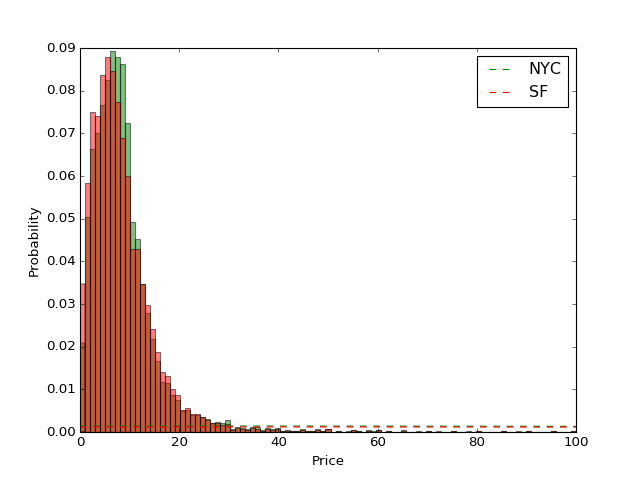
\includegraphics[width=6cm, height=4cm]{dist_sf_nyc_prices}
      \caption{Distribution of the prices in NYC and SF}
      \label{fig:price_dist}
   \end{figure}

This gave us evidence to keep on analyzing all the dataset together. 

In the text, we made a tokenizer that deleted some punctuation signs and that lower cased all the input text. The maximum length of the text was 185, but we decided to cut it to 95th percentile (23 words as limit).

For all our runs, the whole data set of restaurants item's price was split into training(80\%), validation (10\%) and testing(10\%) set randomly, considering that the proportion of observations per city will be the same due to randomness. 

\section{Modeling Framework}
\subsection{Some definitions}
Before explaining our protocol, we give some brief definitions about the tools that will be used.
\paragraph{Word Embedding}
Distributed representation of words are widely used nowadays, they are ubiquitous in many NLP tasks, as they provide semantic relation between words \cite{hill2016learning}.  A good example is the known neural embedding \textbf{Word2Vec} result of a Google's experiment which trains words against other words that neighbor them in the input corpus. Their approach was based on two techniques, the first predicts the word that is in the middle based on the 4 surrounding neighbors which is known as Continuous Bag of Words. The second model is actually the reverse process, to predict the words around a specific one known, called Skip-gram \cite{mikolov2013distributed,mikolov2013efficient}. 

It is common to include the embedding matrix as another parameter to train, but it would be possible that fixing a pre-trained matrix or using it as a start point could bring better results. So, for some experiments, we'll use the pre-trained Word2Vec inputs, as they are available online (\url{https://deeplearning4j.org/word2vec}). There are 3 million vectorized words which have a dimension of 300.  

\paragraph{Neural Networks}
Neural networks (deep learning) have started to be used in NLP for a while now. Most of them are used in tasks such as sentiment analysis, POS tagging, and machine translation tasks \cite{cho2015natural}. 

One of the most used neural networks are the recurrent ones: Long Short Term Memory and Gated Recurrent Unit \cite{cho2015natural} as they don't suffer from vanishing or exploding gradient problems. A huge advantage of GRU and LSTM is that they capture the sentence sequence dynamics, therefore it is possible to get more insights (semantically and syntactically) of the whole text \cite{gers2000learning,cho2014learning,cho2015natural}.


Most of previous works focused in classes prediction, but what if a continuous target enhances the model? If this is considered, maybe the performance of the model would be better. For, we were encouraged to work with a neural network that takes text as input to predict a continuous target.
There's some literature that suggest working schemes for continuous targets such as in \cite{regneural1991} which uses a statistical framework. Based on material seen in class and on \cite{cho2015natural} we find that by changing the loss function, it is possible to focus in a continuous target. We'll use both, categorical an continuous targets in the neural networks to predict price of a restaurant menu's item.

\subsection{Experimental Protocols Proposed}
As it has been stated, the proposed work just considers text as input (item's descriptions and names) to predict a target which is the price. We planned to launch some experiments considering the embedding type, the type of neural network and the type of target.
\begin{table}[ht!]
\centering
\caption{Experiment setup}
\label{table:experiment-setup}
\scalebox{0.8} 
{\begin{tabular}{|l|l|l|}
\hline
\textbf{Target type} & \textbf{Embedding Type} & \textbf{Neural Nework} \\ \hline \hline
Class & Self-learned & MLP \\ \hline
Class & Self-learned & LSTM \\ \hline
Class & W2V fixed & MLP \\ \hline
Class & W2V fixed & LSTM \\ \hline
Class & W2V initial & MLP \\ \hline
Class & W2V initial & LSTM \\ \hline
Continuous & Self-learned & MLP \\ \hline
Continuous & Self-learned & LSTM \\ \hline
Continuous & W2V fixed & MLP \\ \hline
Continuous & W2V fixed & LSTM \\ \hline
Continuous & W2V initial & MLP \\ \hline
Continuous & W2V initial & LSTM \\ \hline \hline
\end{tabular}}
\end{table}

Regarding the embedding, it was possible to set the initial embedding to random numbers, so that it would be another parameter to estimate. Another option was to make the embedding not trainable so it would be a fixed pre-trained matrix. A third option consisted in a mix of the previous: instead of starting from a random point, the embedding matrix could be trained starting from a pre-trained matrix and learned through the optimization process. As mentioned before, we decided to use pre-trained Word2Vec embeddings(W2V) in the cases pre-trained matrices were needed. 

Another option in modeling was to take into account the order of the words, which is usually captured by a recurrent neural network: a LSTM or GRU. Since we wanted to know if order mattered, we decided to launch a  Multilayer Perceptron (MLP) and a LSTM based model for the experiments. 

Finally, we had to decided how was the price target going to be predicted. As it has been stated in the previous section, we'll work with two types of target. The target (natural considered as continuous) was group in 10 groups, making steps of \$5 dollars. This selection was made in order to try to capture the tail of the distribution, given that if percentiles were chosen steps between groups may be too short. 

To give another point of view and to make our experiments comparable, we decided to use a continuous target by setting the loss function to a squared loss.

Our final setup can be seen in Table \ref{table:experiment-setup}. 

\subsection{Model Configuration}

All the models are believed to have the default configuration showed in Table \ref{table:def-config}, otherwise the change will be explicitly mentioned.
\begin{table}[ht!]
\centering
\caption{Default Configuration}
\label{table:def-config}
\scalebox{0.8} 
{\begin{tabular}{|l|l|}
\hline
\textbf{Configuration Variable} & \textbf{Value} \\ \hline \hline
BATCH\_SIZE & 64 \\ 
CHECKPOINT\_EVERY & 200 \\ 
DROPOUT\_KEEP\_PROB & 1 \\ 
EMBEDDING\_DIM & 300 \\ 
EVALUATE\_EVERY & 50 \\ 
MAX\_GRAD\_NORM & 5 \\ 
NUM\_EPOCHS & 10 \\ \hline \hline
\end{tabular}}
\end{table}

The optimizer used depended on the model, for MLP Adam Optimizer was used, with a fixed learning rate of 0.001. For the RNN LSTM a Gradient Descent was used using an initial learning rate of 1, and then a decay of 0.5 if no improvement was found. 

Besides all the mentioned details, specifically for the LSTM model, we considered a mean of all the output states ($h_t$). Also, for MLP we took the mean of all the embedding vectors.

\subsection{Training and Model Selection}
We trained some models considering all 10 epochs, but most of them were trained with a 4 step early stopping, similar to what's suggested in \cite{cho2015natural}. 

Our metric to evaluate the early stop was based on the loss function in development (validation) set . If in 4 evaluation periods the loss was increasing it meant that the model reached a local optima, and the run would stop. 

All of our runs were done in a HPC server requesting around 32GB of RAM and 1 GPU unit, and depending on the experiment it could take from an hour to 24 hours to finish. 

\subsection{Evaluation}
Depending on whether the model was continuous or 10-class, it had a different loss function. Therefore, for the classes model we used accuracy as the main indicator to see how well the model was performing. The loss in this case was set to use a cross entropy (having behind it a 10 class categorical distribution). 

For the continuous model our performance metric was the mean squared error and the mean absolute error, using as loss a squared difference L2-norm as stated in \cite{cho2015natural}.

Furthermore, in order to have more insights on what our model was driven by, we decided to look at the resulting embedding matrix and see how words affected the price prediction. For the former, using t-SNE (with PCA component) to reduce dimensionality to 2D helped us to plot the embedding (more details in \cite{maaten2008visualizing}). Also, for the latter, we adapted a script to predict interactively prices, this will help us to understand the influence of words. The objective here was to see if our models capture the relations explained in the state-of-the art literature mentioned in part 2.

\section{Results}
Results running all the epochs are shown in Figure \ref{fig:lstm_10ep}.
 
   \begin{figure}[thpb]
      \centering
      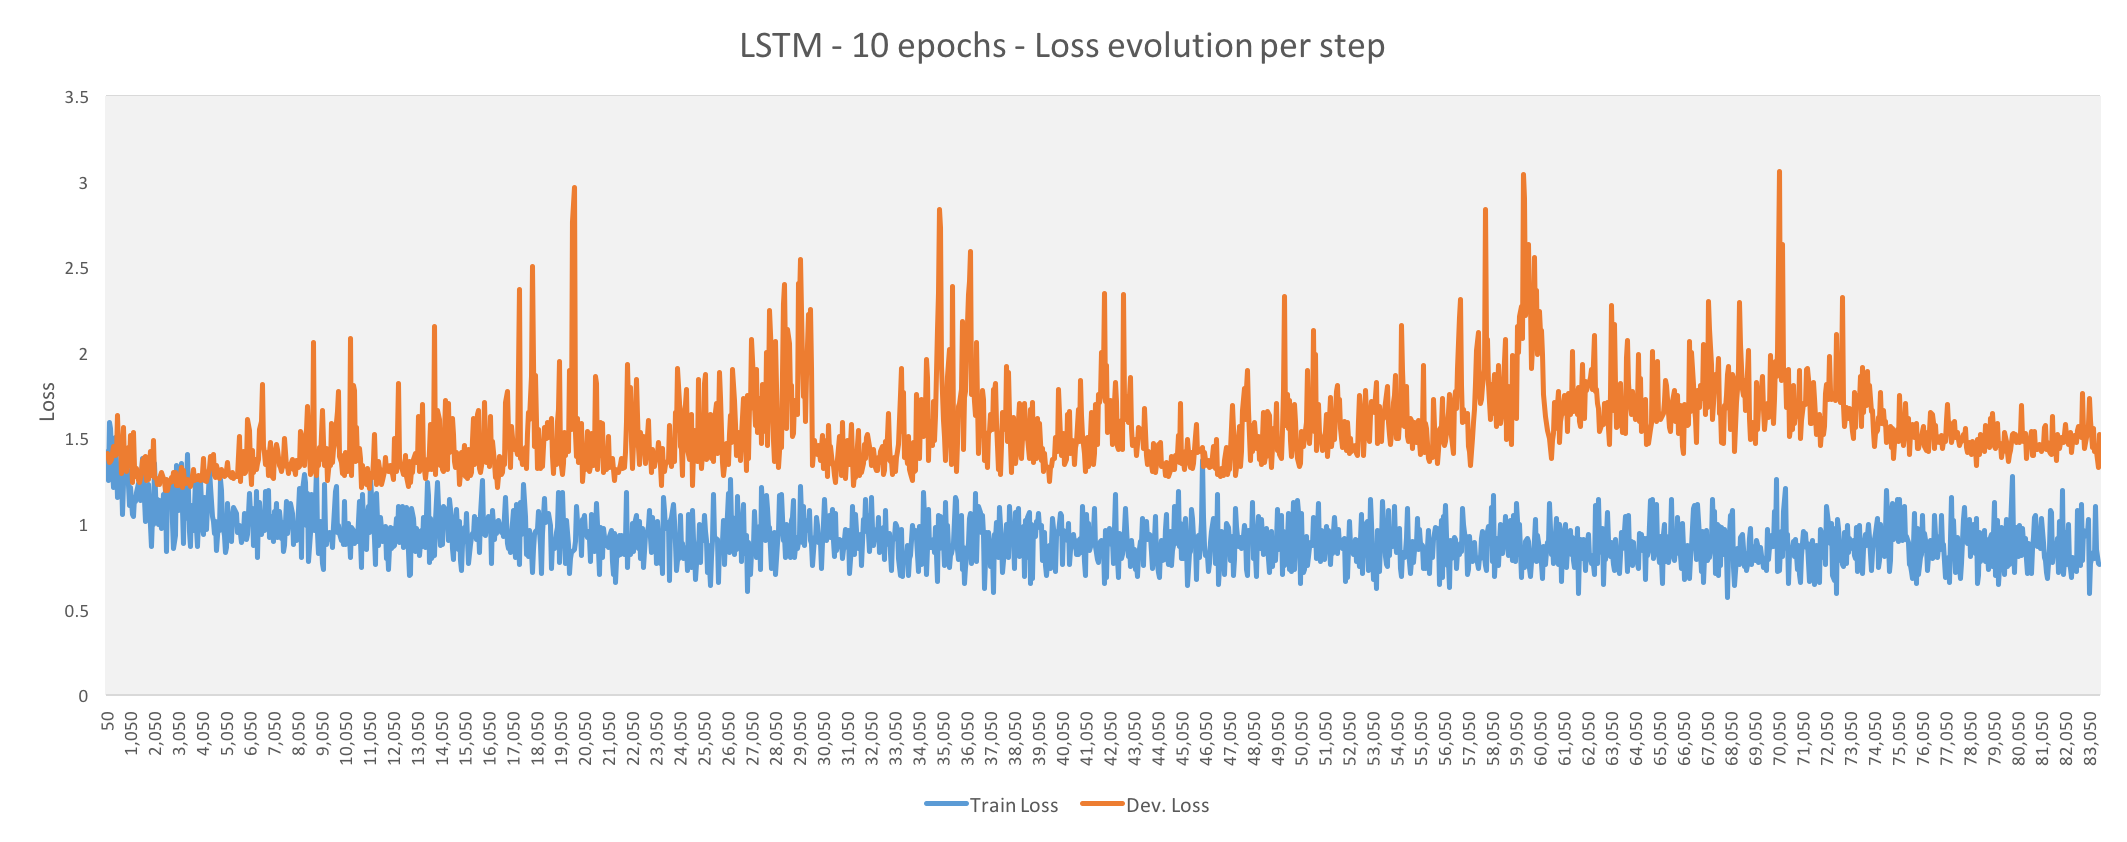
\includegraphics[width=8cm, height=5cm]{lstm_10ep}
      \caption{Distribution of the prices in NYC and SF}
      \label{fig:lstm_10ep}
   \end{figure}

We had a bunch of models to select from each protocol that we decided to try, since randomness of the batches affected all them and we wanted to ensure that the result converged. The best among all our results per category are shown in Table \ref{table:summary-results}.  The indicator column refers to accuracy in case of class target model and Mean Absolute Error, for continuous target.

\begin{table*}[htp!]
\centering
\caption{Best results by protocol. Test Indicator MAE (cont)/ Accuracy (classes)}
\label{table:summary-results}
\scalebox{0.8} 
{\begin{tabular}{|l|l|l|l|l|l|l|l|}
\hline
\textbf{Target type} & \textbf{Embedding Type} & \textbf{Neural Network} & \textbf{Training Loss} & \textbf{Dev. Loss} & \textbf{Test Loss} & \textbf{Test Indicator}  &\textbf{Steps Conv.} \\ \hline\hline
Class & Self-learned & MLP &1.011&	0.94&	0.948&0.627  & 18,800\\ \hline
Class & Self-learned & LSTM & 1.789&	1.823&	1.822&0.3938& 25,600 \\ \hline
Class & W2V fixed & MLP &0.925&	1.133&	1.154&0.532& 64,850 \\ \hline
Class & W2V fixed & LSTM & 1.584&	19.866&	7.699&0.1023& 8.600 \\ \hline
Class & W2V initial & MLP & 0.909&	1.021&	1.01&0.564&  14,200 \\ \hline
Class & W2V initial & LSTM & 1.613&	7.279&	3.462& 0.201 & 48,750\\ \hline
Continuous & Self-learned & MLP &32.03 &   113.83 & 150.497& 3.73 & 43,800\\ \hline
Continuous & Self-learned & LSTM & 23.86 &116.31    & 151.94 & 3.72& 2,500 \\ \hline
Continuous & W2V fixed & MLP & 16.83 & 122.50 &158.79    & 4.00 & 9,700\\ \hline
Continuous & W2V fixed & LSTM & 22.35 & 138.03   &174.39  & 4.60&1,750  \\ \hline
Continuous & W2V initial & MLP & 18.27 & 125.57 &161.86    & 3.98 & 7,100\\ \hline
Continuous & W2V initial & LSTM & 11.22 &112.02& 149.59 & 3.50 &9,150 \\ \hline \hline
\end{tabular}}
\end{table*}

For the best 10-class model MLP, a confusion matrix is plotted to see in which groups our model fails to classify. 

   \begin{figure}[hb!]
      \centering
      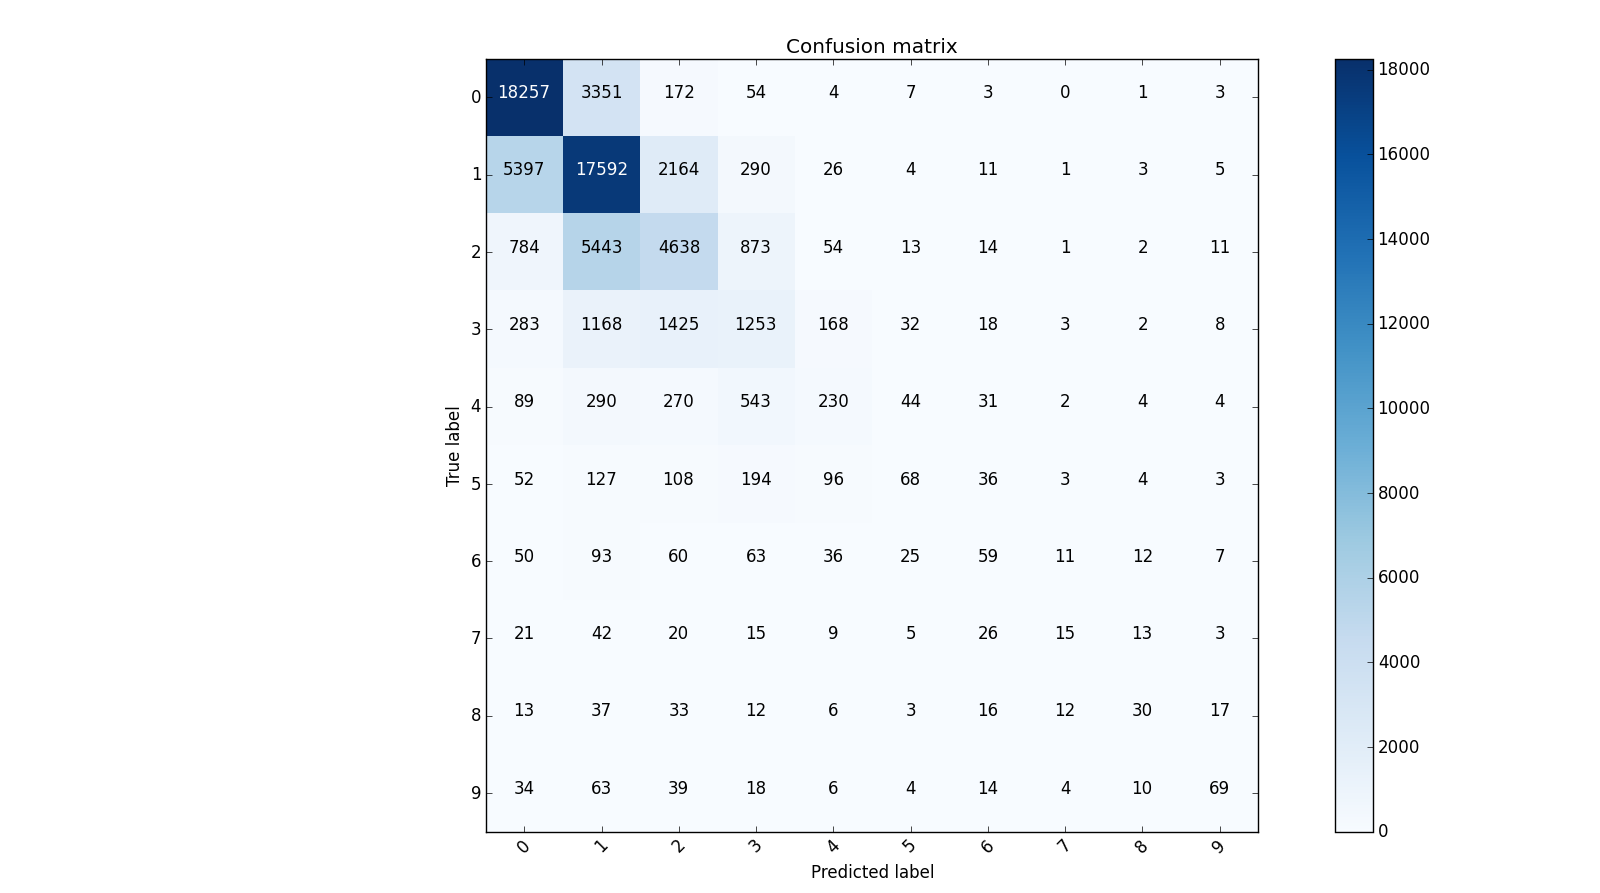
\includegraphics[width=9cm, height=5cm]{confusion_matrix}
      \caption{Confusion - MLP 10 Classes}
      \label{fig:lstm_conf}
   \end{figure}
   
As part of the evaluation, in order to understand more about the model, we chose top 100 words in frequency of a self-learned embedding. The chosen model was the best Recurrent (LSTM) 10 classes, whose projected embedding in 2D (for the most used $300$ words) is displayed in Figure \ref{fig:lstm_emb}.

    \begin{figure}[ht!]
      \centering
      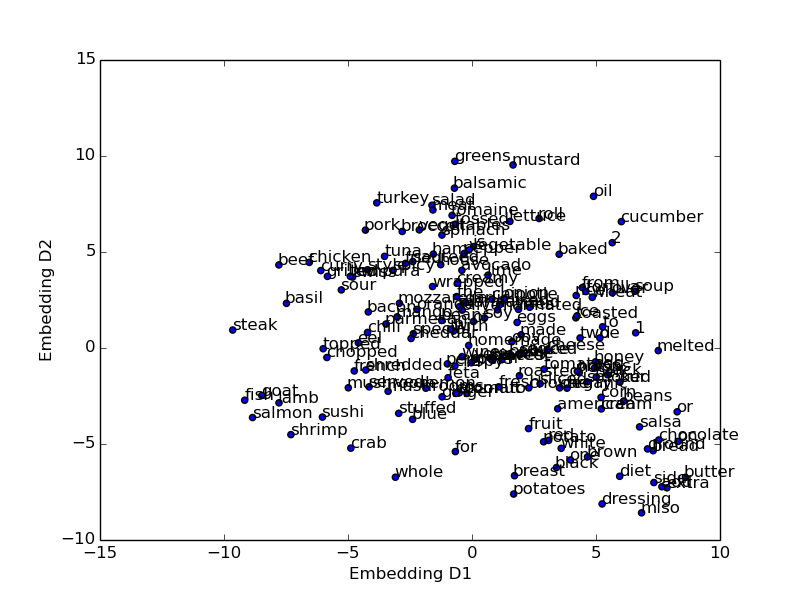
\includegraphics[width=8cm, height=5cm]{Classes300words}
      \caption{Embedding Matrix Projected - LSTM Classes}
      \label{fig:lstm_emb}
   \end{figure}
   
Finally, we evaluated a couple of models with our interactive prediction code. We tested some phrases found on \cite{jurafsky2014language} and some of our own to see how our models reacted.  The results of this evaluation are displayed in Table \ref{table:interactive} 


\section{Analysis}

From Figure \ref{fig:lstm_10ep}, we can conclude that running 10 or more epochs may lead to better results, but the time and resources invested may not worth the increase in performance indicators. Therefore, using an early stop was a good idea. 


When analyzing the class model, we find that running a MLP gives better results compared to the LSTM. We think that this may be due to the quantity of observations that are in the last (more expensive) categories which is also visible in the confusion matrix displayed in Figure \ref{fig:lstm_conf}. However, this would have also affected the MLP, which does not seem the case. So, we begun to think that maybe one LSTM layer did not help capture the dynamics, so making a deeper neural network with regularization (dropout vertically) might alleviate the problem. 

Another interesting thing to notice for classes, is the fact that using pre-trained vectors as Word2Vec worsen the results,even more if it was set to be fixed. This may be because words related to food that are in any WWW page, do not necessarily entail a relation between price. Furthermore, the fact that there are few observations in some classes may affect as well. So, semantical approximation is not enough, we need to consider the price influence too if we want to predict it accurately.


In the case of the continuous model, Table \ref{table:summary-results} shows that the best model is given by an LSTM trained with a initial Word2Vec matrix. This was expected, given that LSTM recovers dynamic relations regarding order. Also, these models seem not to be so affected by the heavy tail (they'll predict the mean as the "default" result).


For this model it is possible to compare results (Mean Absolute Error) with the ones found in \cite{chahuneau2012word}. Their model reached a 3.19  MAE considering a greater data set using up to 3-grams, while ours reached a 3.5 in test set using just SF and NYC menu's description LSTM cells. This means that there is still a gap that could be filled by using more data and by making the neural network deeper.



Which type of model would be better to use? From our analysis, we can say that the continuous target type lead to good results if the (real) price is close to the mean or median. Although, the more the price deviates from the mean, and goes to the tail of the distribution, the worst the prediction is. This may be kind of obvious, but we saw that class model predicts better some values of the tail. So, the selection of the model depends on what you want to do.

The classes model does perform better in predicting expensive dishes (see Figure \ref{fig:lstm_conf}) than the continuous one. The performance for both models in general still seems poor for higher prices, this is likely to be due to the skewness: there is under representation of the tail prices.



Our models also allowed us to check relationship between words by analyzing the embedding plots (t-SNE). Despite the MLP being the best class model, we decided to plot the embedding of the best LSTM to prove that it still gives insights about the semantic relation of words used in a dish description and the price charged for it.

In Figure \ref{fig:lstm_emb} it is possible to see that ingredients are grouped both by their kind and by their price. A good example is the seafood group, they're in the left bottom corner of the graph: fish, crab, sushi, salmon, shrimp, etc. However, one can see that the most expensive seafood are on the top of that group. Another example is the meat group which is in the upper mid part of the plot. Turkey, pork, beef, chicken  are together, but it is possible determine which is cheaper (chicken). Considering the two groups mentioned it is interesting to notice that some kind of more refined  meats (such as goat and lamb) cluster closer to the expensive fish group, meanwhile tuna (usually one of the cheapest kind of fish) cluster along with the other kind of meats. This shows that the price feature in the embedding representation is more important than the more intuitive relations.

We also noticed that some adjectives used to describe cheap food (such as "freshest") tend to be in the upper half of the plot, meanwhile the one that are used for more expensive dish (such as "whole") are in the bottom.

More in general we noticed that the embedding representation enclose interesting relationship between words used in restaurant menus that can be further explored, for example using some non linear clustering techniques such as spectral clustering.

In order to analyze word effects on the price, we used our interactive tool and selected a few examples. As pointed out before, some of them were extracted from \cite{jurafsky2014language} and the rest were examples of our own.  In Table \ref{table:interactive} are predicted results from some menu phrases. 

\begin{table*}[ht!]
\centering
\caption{Interactive Prediction Examples}
\label{table:interactive}
\scalebox{0.8} 
{\begin{tabular}{|l|l|l|}
\hline
\textbf{Menu Description} & \textbf{Classes} & \textbf{Continuous} \\ \hline \hline
(1) imported 18 month aged prosciutto, tomato, mozzarella \& basil & 2 - (10-15{]} & 11.63 \\ \hline
prosciutto, tomato, mozzarella \& basil & 1 - (5-10{]} & 10.99 \\ \hline
imported 18 month aged ham tomato, mozzarella \& basil & 1 - (5-10{]} & 10.79 \\ \hline \hline
(2) crisp golden brown belgian waffle with fresh fruit & 1 - (5-10{]} & 9.18 \\ \hline
belgian waffle with fresh fruit & 0- (0-5{]} & 9.9 \\ \hline
crisp golden brown belgian waffle with fruit & 1 - (5-10{]} & 8.89 \\ \hline
crisp golden brown  waffle with fruit & 1 - (5-10{]} & 8.84 \\ \hline \hline
(3) eggs au beurre noir & 1 - (-10{]} & 9.92 \\ \hline
eggs with black butter & 0- (0-5{]} & 9.77 \\ \hline \hline
(4) enchiladas & 0- (0-5{]} & 9.27 \\ \hline
enchiladas verdes with cheese & 1 - (5-10{]} & 9.45 \\ \hline \hline
\end{tabular}}
\end{table*}

For (1) the original description included italian words making emphasis in the abroad origin, resulting in a 10-15 dollar class prediction. If we remove the word "imported", the class decreases one group. In the continuous case the same happens. If we translate "prosciutto" to ham, the price also reduces, and the continuous prediction shows this has a larger effect as the price decreases almost a dollar.

Example (2) predicts a middle price product that originally has a lot of filler words and adjectives. If we make the phrase simpler, continuous model tells us that the price would increase, but the classes model mentions a decrease in price. This is an interesting finding, as literature suggests that with less filler words, the price should increase. The difference in the class prediction may be due to the length of the new description, as we've seen that usually longer simple phrases give a more expensive prediction. The rest of examples, suggest what was said by Jurafsky that less vocabulary is usual of cheap restaurants. 

The third (3) example uses a lot of french words keeping a simple but descriptive structure, which makes a high price prediction according to the categorical model. If the description is translated, the price decreases, this effect is seen in both classes and continuous models. 

Finally, in our example (4), we use a mexican plate. If we write it in one word, the price is really low, but if it is more descriptive (not using a lot of filler words) the price increases for both models.

All these examples show that our models capture some of the previous studies' conclusions. Filler words and over use of adjectives tend to decrease the price, but if foreign vocabulary is used the plate is likely to be more expensive. It's not a good idea to just name the dish, a small description helps in making the plate more appealing. 



\section{Conclusions}
The results obtained with our continuous model are comparable to the one in \cite{chahuneau2012word}.  And, even though the MAE indicator is slightly worse for our models, we believe that this could be easily improved by using a bigger data set and with a better tuning of the neural network, as we tried several iterations but of only a couple of architectures. Moreover, we believe that our models are better suited for interpretation analysis, mainly because of the trained word embedding and the semantic relation (also with price) that its use brings along.


Another point we found is that our models captured intuitive and state-of-the-art findings, we're able to distinguish which words characterize low and high menu's prices. Filler words and adjectives tend to be used in mid and low-cost restaurants to describe their plates. While a foreign vocabulary is usually used more in high-cost restaurants, with simpler and direct words. These findings were also mentioned by Jurafsky in both of his works \cite{jurafsky2014language,jurafsky2016bordieu}, implying that there is relation between food description and socioeconomical background.



%But also because the trained neural network allow to predict 

\paragraph{Limitations}
While training our continuous model, we noticed that it tends to predict the mean of the distribution (around 8.9). We believe that this is due to the heavy tail the distribution holds, meaning that if this model is to be used an adjustment in the right tail must be done. 
\paragraph{Future Work}
Some questions that arose to both of us was: what exactly makes Word2Vec to give such poor results for classes and good results for Continuous target? How is that LSTM worked in continuous but not in classes models? We're really curious about what leads the models to behave as they have. Maybe the depth of the network? or was it the distribution?

The first future work we would do is try to test more configurations: number of layers, depth of the network mainly; and add regularization (dropout) as they could generate changes in the final performance indicator 

Another improvement would be to use some technique that allows to adjust the tail, as it tends to center the values around the mean, maybe a resampling would help.

Also, we used word embedding as word representation to capture the syntactic relations (with price) between words. However, it is possible to use sentence embedding to see if these capture more and therefore brings a better model \cite{hill2016learning}. 




\section*{Acknowledgments}
We'd like to thank Prof. Bowman for allowing us to the explore relationship between text in food descriptions and prices using neural networks, and for his advice throughout the project.

Also, we appreciate Tensorflow and $dennybritz$ (github account) for making their code public, as we based our code in theirs. 

\section*{Collaboration Statement}
MC scrapped NYC's menus, while LQO did the SF ones. Both designed the experiments and the runs were split: MC was responsible of the continuous models and LQO of the classes. The paper was written and reviewed by both. 

\bibliography{naaclhlt2016}
\bibliographystyle{naaclhlt2016}



\end{document}